\begin{enumerate}[label=\thesubsection.\arabic*, ref=\thesubsection.\theenumi]
\item 
Prove that the three points (3,  0),  (– 2,  – 2) and (8,  2) are collinear.
\label{chapters/11/10/2/20}
	\\
	\solution 
			From \eqref{eq:line-rank-2},
the collinearity matrix can be expressed as
 \begin{align}
			    \myvec{-5 & -2
			    \\
			    5 & 2 }  
			    \xleftrightarrow[]{R_2 \leftarrow {R_1 + R_2}}
			    \myvec{	    -5 & -2  
			    \\
			    0 & 0}  
\end{align}
which is a rank 1 matrix. The above process is known as row reduction, where we try to obtain zero rows in the matrix using arithmetic operations.  The number of nonzero rows in the row reduced matrix (also known as {\em echelon form})
is defined as the rank.
		\figref{fig:11/10/2/20}.
	\begin{figure}[H]
		\centering
 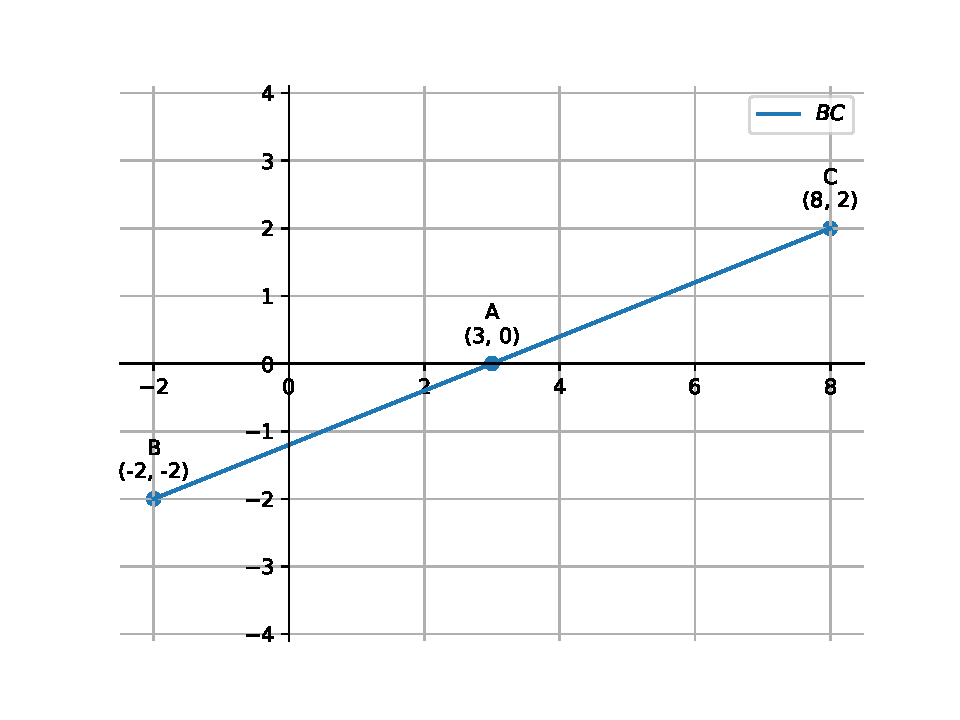
\includegraphics[width=0.75\columnwidth]{chapters/11/10/2/20/figs/fig.pdf}
		\caption{}
		\label{fig:11/10/2/20}
  	\end{figure}

\item Show that the points $\vec{A}(1, 2, 7),  \vec{B}(2, 6, 3)$ and $\vec{C}(3, 10, -1)$ are collinear.
	\\
		\solution The matrix
\begin{align}
	\myvec{\vec{B}-\vec{A}& \vec{C}-\vec{A}}^\top 
	= \myvec{1 & 4 & -4 \\ 2 & 8 & -8}
	\\
	\xleftrightarrow[]{R_2 = R_2 - 2R_1}
	 \myvec{1 & 4 & -4 \\ 0 & 0 & 0}
\end{align}
which has rank 1.  Using 
			\eqref{eq:mat-rank-t}, 
			 we conclude that the given points are collinear.
\item Determine if the points $(1, 5), (2, 3)$ and $(-2, -11)$ are collinear.
\item Show that the vectors $2\hat{i}-3\hat{j}+4\hat{k}$ and $-4\hat{i}+6\hat{j}-8\hat{k}$ are collinear.
\item Show that the points (2,  3,  4),  (–1,  –2,  1),  (5,  8,  7) are collinear.
\item In each of the following,  find the value of $k$,  for which the points are collinear.
\begin{enumerate}
\item $(7,  –2),  (5,  1),  (3,  k)$
\item $(8,  1),  (k,  – 4),  (2,  –5)$
\end{enumerate}
		\label{10/7/3/2}
\item Find a relation between $x$ and $y$ if the points $(x,  y),  (1,  2)$  and  $(7,  0)$ are collinear.
\item If three points $(x,  -1),  (2,  1)$ and $(4,  5)$ are collinear,  find the value of $x$.
\label{chapters/11/10/1/8}
\item If three points $(h,  0),  (a,  b)$ and $(0,  k)$ lie on a line,  
show that 
\begin{align}
\frac{a}{h}+\frac{b}{k}=1
\end{align}
\label{chapters/11/10/1/13}
\item Show that the points $\vec{A} (1,  -2,  -8),  \vec{B} (5,  0,  -2)$ and $\vec{C} (11,  3,  7)$ are collinear,  and find the ratio in which $\vec{B}$ divides $AC$.
\item lf the points $\vec{A}(1, 2), \vec{0}(0, 0)$ and $\vec{C}(a, b)$ are collinear, then find the relation between $a$ and $b$.
	\item Point $ (-4, 2)$ lies on the line segment joining the points $ \vec{A}(-4, 6)$  and  $\vec{B}(-4, -6)$.
 \item The points $(0, 5), (0, -9)$ and $(3, 6)$ are collinear.
\item Points $\vec{A}(3, 1),  \vec{B}(12, -2)$  and  $\vec {C}(0, 2)$ cannot be the vertices of a triangle.
\item Find the value of $m$ if the points $(5, 1), (-2, -3)$  and $(8, 2m)$ are collinear.
\item Find the values of $k$ if the points $\vec{A}(k+1, 2k), \vec{B}(3k, 2k+3)$ and $\vec{C}(5k-1, 5k)$ are collinear.
\item Using vectors,  find the value of $k$ such that the points $(k, -10, 3)$,  $(1, -1, 3)$  and  $(3, 5, 3)$ are collinear.
\item The points $\vec{A}(2, 1)$,  $\vec{B}(0, 5)$,  $\vec{C}(-1, 2)$ are collinear.
\item The vectors $\lambda\hat{i}+\lambda\hat{j}+2\hat{k}$,  $\hat{i}+\lambda\hat{j}-\hat{k}$ $\text{ and }$ $2\hat{i}-\hat{j}+\lambda\hat{k}$ are coplanar if
	$\lambda=$
\item Show that the points $(-2, 3, 5),  (1, 2, 3)$ and $(7, 0, -1)$ are collinear.
\item Show that points $\vec{A}(a,  b+c),  \vec{B}(b,  c+a),  \vec{C}(c,  a+b)$ are collinear.
\item Show that the points $\vec{A}(2, -3, 4),  \vec{B}(-1, 2, 1)$ and $\vec{C}(0, \frac{1}{3}, 2)$ are collinear.
\item Are $\vec{A}(3, 1), \vec{B}(6, 4)$ and $\vec{C}(8, 6)$ collinear?
\item Find the values of $k$ if the points $\vec{A}(2, 3),  \vec{B}(4, k)$ and $\vec{C}(6, -3)$ are collinear.
\item Three points $\vec{P}(h, k),  \vec{Q}(x_1, y_1)$ and $\vec{R}(x_2, y_2)$ lie on a line. Show that $(h-x_1)(y_2-y_1)=(k-y_1)(x_2-x_1)$.
\item Show that the points $\vec{P}(-2, 3, 5),  \vec{Q}(1, 2, 3)$ and $\vec{R}(7, 0, -1)$ are collinear. 
\item Prove that the three points $(-4, 6, 10),  (2, 4, 6)$ and $(14, 0, -2)$ are collinear.
\item Show that the points $\vec{A}(-2\hat{i} +3\hat{j} +5\hat{k}),  \vec{B}(\hat{i}+2\hat{j} +3\hat{k}$ and $\vec{C}(7\hat{i} -\hat{k})$ are collinear.
\item Show that the points $\vec{A}(2,  3,  -4),  \vec{B}(1,  -2,  3)$ and $\vec{C}(3,  8,  -11)$ are collinear.
\end{enumerate}
